Objectives are either based on diff metrics or on distance metrics.


Search based approaches

MOMot - maybe mention MOMoT just in the evaluation section?


 All experiments use the same input and output models, the same transformations, the same solution length and the 
same optimization algorithms and only differ in the fitness functions used in these algorithms. 
The exact Pacman and Petrinet cases have been freshly created for this evaluation, but are commonly used in the graph transformation world.
In the past, the Refactoring case has been used to evaluate different algorithms for MoMOT in the past, where all algorithms optimized the same fitness function. How, this case is used to evaluate the same algorithm with different fitness functions.


\subsection{Objective}

As our main goal is to compare different fitness functions in terms of their impact on search processes, we want to answer two research questions:

\begin{itemize}
	\item \textit{RQ1 - Search Space Exploration}: Is there a significant difference in the solutions found by applying each fitness function?
	\item \textit{RQ2 - Search Time}: Is there a significant difference in the number of iterations required to get good solutions?
	%Senseless - you can easily define simple generic model distance functions which are much faster, e.g. by just mapping things to feature vectors
	%EMFCompare might be really slow, but that isn't everything
	%\item \textit{RQ3 - Search Time}: Is there a significant difference in the time 
\end{itemize}

We answer these research questions by measuring several properties of the final and intermediate results during each experimental run.
In particular, to answer RQ1, we compare the final solutions, while we comare the intermediate results to answer RQ2.

\subsection{Experiment setup}


We evaluate these research questions with three MoMOT case studies. Each case study consists of a single domain model and multiple henshin transformations.
The \textit{Pacman} case study has been introduced in Section~\ref{sec:motivating}. The \textit{Petrinet} case study simulates a Petrinet with multiple tokens which can be in different places. A token can be transferred to another place by firing transitions. The \textit{Refactoring} case study, as found in \cite{?}, is about performing refactoring operations like extracting superclasses or pushing up attributes to a model containing classes and attributes.
For each case, we randomly generated multiple test input and output models as outlined in following paragraphs.

\begin{table}
\begin{tabular}{|c|c|c|c|}
\hline 
 & \textbf{Pacman} & \textbf{Petrinet} & \textbf{Refactoring} \\
\hline
\textbf{Rule count} & High & Low & Medium \\
\hline
\textbf{Rule complexity} & Low & Low & High \\
\hline
\textbf{Solution length} & High & High & Low \\
\hline
\textbf{Structural changes} & No distance changes & - & Distance changes \\
\hline
\end{tabular}
\end{table}

The case studies have selected as they differ in terms of rule count, rule complexity, and expected solution length as detailed in Table~\ref{tab:casecomp}.
The Petrinet simulation contains only a single rule which can match in many different ways and whose application does not limit its re-execution. Thus, the rule count is low, but the expected solution length is high. In contrast, the rules for Object Oriented Refactoring typically can be applied in a more limited way and applying it typically limits the application even more, yielding a lower expected solution length. The Pacman example is somewhere inbetween as many rules are defined, but they semantically all do the same, which is moving Pacman or a Ghost, but only differ in what happens on specific fields. 
Most importantly, only the Refactoring example contains rules which modify the graph in way which matters for the domain specific distance evaluation. A detailed description of the cases follows in the next paragraphs.


\paragraph{Pacman} The pacman example was described in the previous sections and is thus not explained further here.


\paragraph{Petrinets} 
This example consists of places which may be connected to other places via transitions. A place can have multiple transitions
and each transition can have multiple outgoing states, contributing to a non-determinism in firing the rules.
While places and transitions are modeled as named objects, tokens are not objects, but are just modeled as attribute values.


\begin{figure}
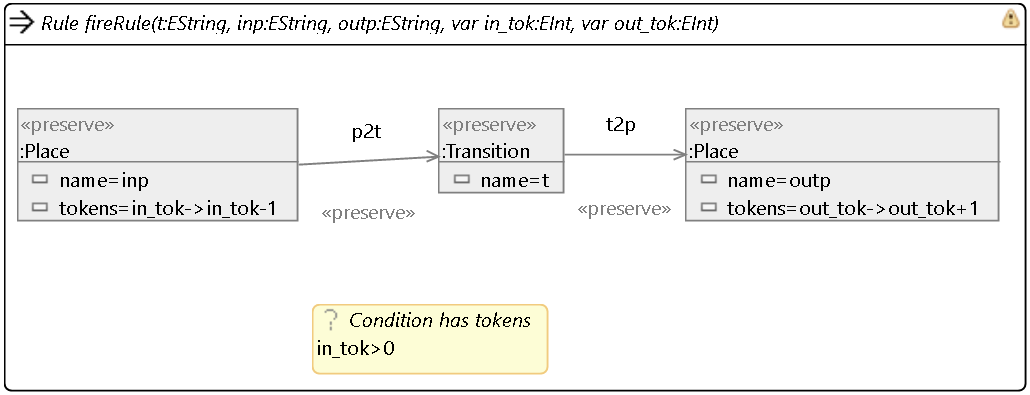
\includegraphics[width=0.8\textwidth]{images/firetransition.png}
\caption{A transition can fire if there is at least a single token in the source place}
\label{fig:firerule}
\end{figure}

There is only a single rule \textit{fireRule} as shown in Fig.~\ref{fig:firerule} which allows to move a single token from a place to another place. 
As usual for MoMOT, the parameters of the rule uniquely identify the rule match. Even though the model is simple, the number of models generated
by applying this rule multiple times can be huge, especially if multiple tokens are used.

\paragraph{Object-oriented refactoring}

This example~\footnote{Also see \url{http://martin-fleck.github.io/momot/casestudy/class_restructuring/} for a detailed description}, which was initially taken from the TTC 2013, contains entities with named, typed properties and generalizations. 
Originally, it was used as optimization problem to reduce the number of attributes and entities in a system. However, in this paper
we want to find a way to refactor a system in a particular fashion. The three refactoring rules are (a) Pull up attribute, which moves an attribute existing in all subclasses into the superclass, (b) extract super class, which creates a new superclass if an attribute is existing in some, but not all subclasses of a particular class, or (c) create root class, which is the same if the classes do not have any existing superclass.

In contrast to both examples above, this example changes the model structure by adding entities and generalizations and removing properties.



\subsection{Analysis}

In the following, we describe the results of the experiments conducted in terms of the research questions.


While many general distance metrics exists, we opted for an EMF-compare based one as this tool is widely used for differentiating models. In particular, we calculate the difference between two models by counting the percentage of model differences in the whole model.

Initially, we generated 100 examples of pairs of source and target model for each case. As the results for the Refactoring case initially were good, but not statistically significant, we generated 1000 examples for this case as well. While the source model was generated randomly within
certain predefiend parameters, the target model was generated by randomly applying transformations to the source model. 
However, for the Pacman case, we had to add more "`intelligent"' rules to generate sensible target states as typically, randomly applying move operations
just lead to Pacman being killed soon by running into a ghost or just being eaten by a ghost. Here, the rules force Pacman to eat neighboring food when possible and avoiding any ghosts. The search process itself does not use these rules, but just the generic ones.

For each example, only a single run was conducted. Then, the final solutions generated by each run were compared.
A solution is considered better if the number of transformations used to reach the target model is smaller. If a run did 
not produce any transformation sequences matching the target model, this number is considered to be infinite. We did not consider cases where 
the result models were not exactly matching the target model as at least two different distance metrics could be used for that.

To determine which fitness function was better we assumed that if both fitness functions would produce equal results,
there was a 50/50 chance that either fitness function was better for runs which produced differences.
For each example, we calculated the chance that the distance metrics would be as good or better just by chance.
Thus, we can reject the null hypothesis that the domain specific fitness function is not better if this value is below 5\%.

%Values are so low - calculate p exactly!


\subsubsection{Results for RQ1 Search Space Exploration}

\begin{table}
\begin{tabular}{|c|c|c|c|c|}
\hline
 & Generic & Equal & Domain-specific & p-value \\
\hline
Pacman & 1 & 73 & 27 & \textbf{.11E-7} \\
\hline
Petrinet & 26 & 30 & 45 & \textbf{.016} \\
\hline
Refactor (100) & 22 & 47 & 32 & .11 \\
\hline
Refactor (1000) & & & & \\
\hline
\end{tabular}
\label{tab:resultsrq1}
\end{table}

Table~\ref{tab:resultsrq1} shows the differences in the results quality for both approaches. For the Pacman case, we generated 8x8 fields with one Pacman, three ghosts, and 15 food, where all food and all other entities were randomly distributed. The Petrinet case used 10 places and 1 to 2 transitions per place and 1 to 2 outgoing place per transition. Also, the net was initialized with between 2 and 4 tokens. The Refactor case used 6 entities, 1 to 5 attributes per entity, where each name was one of 8 possible names and each attribute name was associated to 1 to 3 types. Also, each entity had a 50\% chance to have a random superclass. 

The Pacman case was rather hard for both fitness functions - all the equal values are due to no solution being found in either case. However, in this instance the domain specific fitness function could show its benefits, as it could solve the problem in 27 cases, while the generic one could only solve it in one case, yielding a significant difference. In contrast, the Petrinet case was rather easy for both algorithms, as most of the equal values were due to both algorithms finding solutions having the exact same quality. Still, the domain specific fitness function allowed us was at least statistically significantly better.


\subsubsection{Results for RQ2 Search Time}

We determined the rate of convergence by storing the solutions found after each evaluation step



%* Linearize quality to make comparable
% - Alternative: Just make "`normal"' comparison in each step?

%* Calculate average solution quality over the course of the runs
% - Save solutions after each step
% - Maybe different distance function implement? Normalize with initial difference
% - Just show it, values ... I am not sure that they would be sensible here

While exact time measurements were not taken, the domain-specific distance function always was faster, sometimes drastically faster,
than the generic EMF-compare based one. 

%- Time: EMFCompare takes longer (difficult to measure reliable, as performance VS solution quality metrics collide)
%- Unexpected: EMFCompare converges faster initially for many models - why?
% * Distance metrics used is EMFCompare ...

\subsection{Threats to validity}

\subsection{Discussion}
The current implementation assumes that M1 and M2 have the same position objects (none are deleted or created). This is too restrictive. Therefore M1 and M2 should be preprocessed by merging their position elements and then use the move distance. One possibility is to use EMFCompare to merge M1 and M2 based on the position elements.

Interestingly, when you run the Pacman test with models/input12missing.xmi and models/targetNoPac.xmi in one signle run, you don't necessarily get always the same sequence of rule applications. That is because p1 can be killed anywhere along the path of g1. 